%%% Results %%%
\chapter{Results and Evaluation} \label{ch:results}
This chapter presents the evaluation of the endorsement model as proposed in
Chapter~\ref{ch:method} based on which the overall system design and
functionality are assessed and final results are presented. It begins by
discussing the relevant threat models and how the endorsement model addresses
them. 

\section{Threat Models}\label{sec:threatModel}
Relevant threat models and how the endorsement system addresses them is
presented in this section. 
\paragraph{Sybil attack:}The endorsement system addresses the Sybil attack by
requiring the endorsers of a peer to have a high ~\ac{TEI} value as well. A
peer can create multiple identities and self-interact to send a large number of
endorsements to direct to themselves. However, being endorsed by a new set of
endorsers (or endorsers with no activity on the network) does not help to get a
higher value as discussed earlier in Section~\ref{sec:interaction}. To overcome
this, a malicious node may try to send endorsements among each other such that
each identity has a significant impact value leading to a better trust score on
the identity they intend to inflate the score of. However, doing so requires
sending many endorsement transactions over to the ethereum network and raises
the cost of operation.   
\paragraph{Whitewashing:} The idea of rewards and punishment as discussed in
Section~\ref{rewardpunishment} aids in lessening a whitewashing behavior. By
punishing the misbehaving nodes in a way that decreases their score made so far
significantly but still preventing the value to be lower than a new user,
whitewashing is addressed. The punishment of a node requires communication with
the transaction network to receive the feedback on a transactional outcome.  
\paragraph{Free riders:} Free riders issue is addressed by requiring the nodes
to have a balanced ratio of outgoing and incoming connections.
\paragraph{Denial of service:} Denial of service is addressed by deploying the
endorsement system on a public, permissionless blockchain network. There is no
way to know a priori the address of a validator node that will be signing the
next block. Therefore, attackers do not know where to direct the attack to
intrude the operation of endorsement transactions. 
\paragraph{Self-promoting and Slandering attack:}The cryptographic functions of
the blockchain solve the possibility of this attack due to lack of data source
authentication or data integrity verification, and once the transaction is
added to the blockchain, the blockchain protocol provides the guarantee of the
immutability of data and offers public verifiability of data. Another reason
this attack is possible is by creating multiple Sybil identities. This is
addressed by the cost of operation to do so, i.e., the account that initiates
the transaction (joining the network or sending endorsements) has to pay the
cost of each operation.   
\paragraph{Malicious collective:}Malicious nodes can form a collective group
and endorse each other until they all have a high \ac{TEI} value to be
considered trustworthy in the endorsement network. The endorsement system
metrics allow the possibility for malicious collectives to be seen as more
trustworthy. The current implementation of the endorsement system does not
address this issue. However, the information available about an entity can be
used, if needed to find out malicious nodes that explicitly interact within
their group. \par
Consider a malicious collective of four nodes, $M = \{A,B,C,D\}$ that endorses
each other. The endorsement system maintains two sets of data for each
participant, one that contains the list of endorsers, and other that contains
the list of endorsees. \par
If $A$ represents the list of endorsers and $A'$ represents the list of
endorsees for the entity $A$, then, we can find the intersection of the sets
$A$ and $A'$ to find out the list of common entities in these two sets. The
elements of this intersection set should represent the entities with whom $A$
has the symmetric trust relation with.  
\begin{equation}
	\begin{split}
	A= \{B,C,D\} \\
	A' = \{B,C,D\} \\
	A \cap A' = \{B,C,D\}
\end{split}
\end{equation}
As we can see that the intersection set includes the same list as the list of
endorsers and endorsees, it is most likely that these entities are forming a
malicious collective to inflate the trust scores of each other. However, this
does not provide enough information to infer that a node is malicious with
certainty. We cannot ignore the possibility that they know each other and the
endorsement interaction is an honest one. The characteristic of trust as being
asymmetric does not invalidate the existence of the symmetric trust, i.e., $A$
trusts $B$ does not imply $B$ has to trust $A$ but it is entirely up to $B$ if
he trusts $A$, and only $B$ knows if the trust relationship is an honest or
malicious one. \par
Hoffman, K., Zage, D. and Nita-Rotaru, C., 2009~\cite{hoffman2009survey}
relates the process of finding the colluding nodes as such to finding a
clique~\footnote{A clique~\cite{cormen2009introduction} in an undirected graph
	$G = ( V,E)$ is a subset $V' \subseteq V$ of vertices, each pair of which
is connected by an edge in $E$.} of a certain size in a graph, which has been
known to be NP-complete and only has heuristic based solutions.  An important
consideration to be taken if one wants to find the intersection of sets of
endorsers and endorsees is that as the size of the sets grows, so does the
computational complexity. Given, the amount of gas that each operation costs,
it does not seem to be a feasible solution for doing this form of computation
on ethereum blockchain. As such, it is recommended to implement it on a
client-side and only make the computation if invoked by the client.

\section{Evaluation of Requirements}
A descriptive approach based on the design evaluation method by Hevner A,
Chatterjee S.~\cite{hevner2010design} is used to assess the system requirements
when relevant, e.g., security and reliability aspects of the system is assessed
based on the information available regarding blockchain and smart contracts to
demonstrate the utility of the system. The system is not only reliant on the
smart contract code and its execution but also on the interaction theory
discussed during the design of the endorsement system. For this, the
endorsement interaction is simulated using the graph simulation tool
neo4j~\footnote{https://neo4j.com/}. The dataset used to simulate the
interaction is taken from SNAP~\cite{snapnets}. The details on the dataset are
presented in Section~\ref{sec:interaction}. Given the time constraints, no form
of structural/unit testing was performed. The purpose of this project was a PoC
design to demonstrate the reputation model as a use case via the use of smart
contracts and blockchain technology. An extensive experiment to simulate a
real-world usage was not performed. However, manual testing was done during
development using ganache~\footnote{https://github.com/trufflesuite/ganache/}
and deployment of contract on a local network. Additionally, front-end was
developed to test contract function calls and communicate with contracts on
blockchain network from the browser itself.  

\section{Fulfillment of User stories and Requirements}\label{fulfillment}
The method to examine fulfillment of user stories and requirement follows the
method used by Hevner's descriptive design evaluation
approach~\cite{hevner2010design}. Table~\ref{table:fulfillment} presents
the motivation for fulfillment of functional requirements. For the relevant
smart contract code, refer to Appendix~\ref{smartcontracts}. 
The fulfillment of non-functional system requirements is discussed below:
\paragraph{Smart contract security:} Solidity~\cite{soliditySecurity}
recommends ordering the contract code as conditions, actions and interactions,
i.e., first make all the necessary checks (e.g., who called the function, if
arguments are in range) and only if these checks pass then perform the actions
that change the state of the current contract. Interaction with other contracts
(calling another contract) should be the last step in any function. Following
this pattern can avoid Re-entrancy bug~\cite{atzei2017survey}, i.e.,
interrupting a function call in the middle of execution and re-entering before
the previous execution is over. The function call can be made by both ~\ac{EOA}
or by a contract address. A maliciously crafted contract can make a function
call repeatedly before the execution of the function ends or throws an
exception which can cause the function to interact in unintended ways. As such,
failing early by making the checks first in a function can avoid such a bug. \par
The contracts written for the endorsement system followed this approach. A
snippet of function to join the network is given by
Listing~\ref{contractsecurity}. As we can see, the "joinNetwork" function
first makes a check to see if the user has already been registered. If the
check fails, then further execution of the function is stopped. Only if the
checks pass then it moves further to remaining parts of the function that deals
with actions to change the state of contract, i.e., change the state of
"joined" for the message sender (new user), add this new user in the list of
participants and increment the number of registered participants. These are
examples of actions that update the state variables of the endorsement
contract. The rest of the contracts function is written following the same
pattern of making checks before changing the state whenever relevant (i.e., any
function call that can change the state). An endorsement contract is a single
contract that performs all the core logic of the endorsement system and
therefore, interaction with other contracts is not required. 
%Based on the recommendations by
%Solidity~\cite{soliditySecurity}, contract function code was ordered as
%conditions, actions, and interactions where relevant. For example, execution of
%a function to join the endorsement network first makes a check to see if the
%user has already been registered. If the check fails, then further execution of
%the function is stopped. Only if the checks pass then remaining parts of the
%function gets executed. Doing so can avoid Re-entrancy bug, e.g., interrupting
%a function call in the middle of execution and re-entering before the previous
%execution is over. The function call can be made by both ~\ac{EOA} or by a
%contract address. A maliciously crafted contract can make a function call
%repeatedly before the execution of the function ends or throws an exception
%which can cause the function to interact in unintended ways. As such, failing
%early by making the checks first in a function can avoid such a bug. 
\begin{lstlisting}[language=Solidity, label=contractsecurity, caption=Function to Join Network] 
	function joinNetwork(string _userName) public{
		//conditions: only allow unregistered participant
		require(!joined[msg.sender]);

		//actions
		joined[msg.sender] = true;
		
		Participant memory newParticipant = Participant({
				identifier: msg.sender,
				name: _userName
        });
		participants.push(newParticipant);
        LogJoinNetwork(msg.sender, _userName);
        numberOfParticipants++;
        participantIndex[msg.sender] = numberOfParticipants-1;
    }
\end{lstlisting}


%The security considerations by
%Solidity~\cite{soliditySecurity} was followed for the contract code. Not all
%the recommendations presented there were relevant for the endorsement contract.
%For instance, recommendations on restricting the amount of ether or patterns
%for sending/receiving ether in a function call is not relevant as endorsement
%contract does not require any function call to include any amount of ether as
%the message value. As part of fail-early principle, the contract function code
%was ordered as conditions, actions, and interactions where relevant. Doing so
%can avoid Re-Entrancy bug. The function call can be made by both externally
%owned account or a contract address in ethereum. A maliciously crafted contract
%can make a function call repeatedly before the execution of the function ends
%or throws an exception which can cause the function to interact in unintended
%ways. As such, failing early by making the checks first in a function can avoid
%such bugs. 
\paragraph{Reliability:}The endorsement interactions and the variables required
to compute the trust score of participants are stored on the public,
permissionless blockchain network. As such, the data and variables of the
endorsement system are publicly verifiable information. The \ac{PoW} consensus
algorithm ensures the immutability of data. As there is no central entity to
add or modify the data, the system is resilient to internal modifications. 
%
%This requirement relates to the immutability of data
%stored on the blockchain network which is ensured by~\ac{PoW} consensus
%algorithm. The reputation data is stored on a public, permission less
%blockchain network which allows any node to commit a block of transactions to
%the blockchain. A validator node collates the list of transactions into a
%block. A malicious node that intends to double spend a transaction can do so by
%solving the cryptographic puzzle in parallel with the rest of the network. If
%the malicious does not broadcast the solved blocks to the network and instead
%keeps solving the puzzle in isolation with the network. The transactions that
%the malicious node spent can be included in the blockchain that the network is
%in agreement with currently. After a certain length of blocks has been solved,
%the malicious node can then decide to broadcast his version of blockchain to
%the network.  Blockchain protocol ensures that the network switches to the
%longest chain in the event of a fork. Since the malicious node is in the race
%with rest of the network, this form of attack is only possible if the malicious
%node owns more than 51\% of the hashing power compared to the rest of the
%network. As long as honest nodes control half of the network, the~\ac{PoW}
%mechanism ensures an immutable record of transactions to be stored in the
%blockchain.
%
\begin{center} \label{table:fulfillment} 
	\begin{table}
		\begin{tabular} {| l | l | p{9cm} | }
		\hline
		\textbf{User}  & \textbf{Requirement Id}   & \textbf{Motivation for fulfillment} \\
		\hline
		\multirow{2}{*}{Endorser} & R1 & Any registered participant can make a
		call to endorse() function to send an endorsement to other registered
		participants on the network. 
		\\\cline{2-3} 
		& R2  & Any participant in the list of endorsers for another
		participant $A$ can call removeEndorsement() function to the address of
		$A$.
		\\\cline{2-3}
		& R3 & The call to endorse() function updates the state variables
		\ac{nEG} and the list of endorsees for the endorser. It also invokes
		updateEndorsee() function to update the information (\ac{nER}, list of
		endorsers) of endorsee accordingly. 
		\\\cline{2-3}
		\hline
		\multirow{2}{*}{Endorsee} & R5.& The call to editProfile() function
		allows participants to edit their stored pseudonym.
		\\\cline{2-3}
		\hline
		\multirow{2}{*}{other users} & R4.1 & Anyone can make a call to
		computeImpact() function to get the final computed score of the
		participant based on their account identifier.
		\\\cline{2-3}
		& R4.2 & Anyone can make a call to joinNetwork() function and become a
		registered participant of the network immediately.  
		\\\cline{2-3}
		\hline
	\end{tabular}
	\caption{Fulfillment of User stories and Requirements for Endorsement PoC}
\end{table}
\end{center}
\vspace{-15mm}
\paragraph{Trust metrics correctly describe the actual trust of the nodes:}The
fulfillment of this requirement is assessed by simulating an interaction graph
and analyzing different scenarios in the network. The
Section~\ref{sec:interaction} presents the details regarding this requirement. 
%%%%%%%%%%%%%%%%%%%%%%%%%%%%%%%%%%%%%%%%%%%%%%%%%%%%%%%%%%%%%%%
\section{Interaction graph} \label{sec:interaction}
For the simulation of user interaction in the endorsement network and the
resulting impact value, a real-world data set was used. The dataset was
extracted from Bitcoin Alpha trust~\footnote{https://alphabtc.com/blockchain/}
weighted signed network which is a who-trusts-whom network of people that trade
on Bitcoin Alpha platform. Participants on this network rated each other on a
scale of -10 to +10 where negative value represented total distrust whereas
positive value represented total trust. It consisted of 3,783 nodes that made
24,186 edges out of which 93\% of the edges were marked as positive
edges\cite{kumar2016edge}.  The available information in the dataset for all
the nodes was source, target, rating, and timestamp, all of which are essential
information for the endorsement network. 
\begin{figure}
	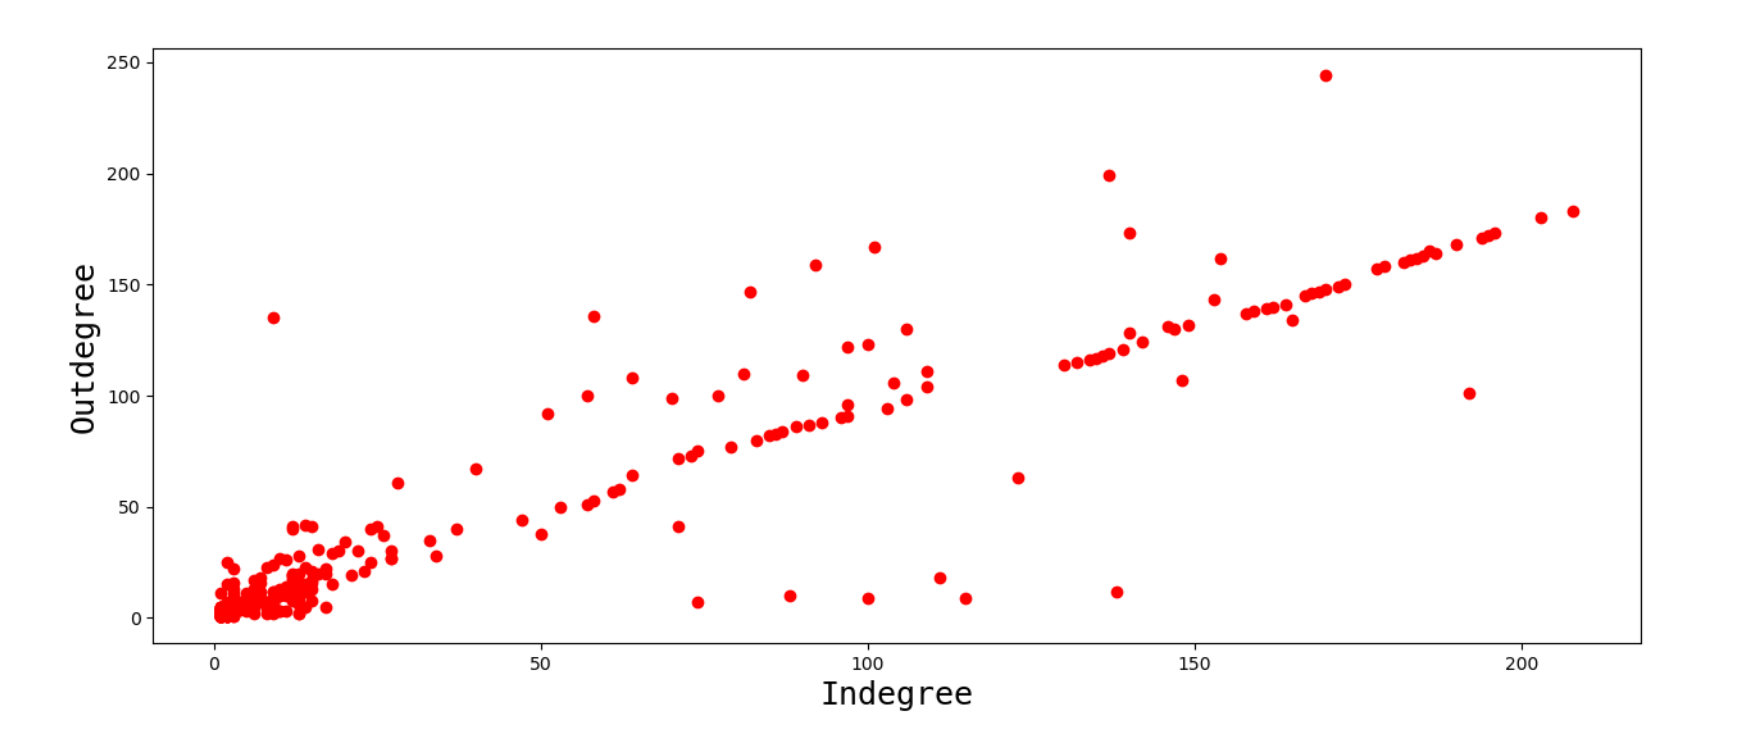
\includegraphics[width=0.95\textwidth]{Images/in_out.eps} 
	\caption{Distribution of degree of incoming and outgoing connections} 
	\label{inOut}
\end{figure}
The direction of endorsement is based on the source and target information.
The timestamp information can help to decide on the order of transaction
occurrence in the network. This information is particularly interesting for
anomaly detection algorithm such as Net flow rate convergence as discussed in
\cite{buechler2015decentralized}. Unlike the Bitcoin Alpha network that let
users rate on a scale of -10 to +10 to demonstrate the strength of their trust
towards the users, the endorsement system only considers values from a binary
domain, i.e., a user either endorses a specific claim made by the entity or
does not endorse. There is no range of values to depict the strength or
weakness. For making it more relevant to endorsement interaction, the existing
dataset was filtered only to have edges with a rating above +2. No negative
edges were considered for the endorsement simulation. As a result, the total
number of nodes was reduced to 1677 with 4776 edges. Endorsement model was then
applied to these nodes, and their total endorsement impact was computed based
on their incoming and outgoing connections. 
%The scores along with new findings are presented below: 

\paragraph{Total Endorsement Impact:} \label{par:TEI}This value is based on the
degree of connections (~\ac{nEG}, ~\ac{nER})and ~\ac{TRP} for each node. Out of
1677 nodes, there were 1175 nodes (70\%) that turned out to have a ~\ac{TEI}
score of zero. On examining the nodes, they were found to have only one
incoming or outgoing connections, i.e., the value of~\ac{nEG} or~\ac{nER} was
only one. As such, the \ac{TEI} score of zero was expected because a node would
only be considered for making an impact on the endorsement system if the number
of connections is more than one. The score of zero, in this case, is not
representative of a non-trustworthy node, but a starting node. Thus, we can say
that 70\% of the nodes in this network are new users. This computation leaves
us with only 502 nodes to account for having a considerable \ac{TEI} score. The
distribution of \ac{nEG} and \ac{nER} among the participants of the network is
given by Figure~\ref{inOut}. As we can see in the figure that most of the nodes
have a low incoming and outgoing connection whereas only a few nodes seem to
have a high degree of connections. We can also see a few nodes that have
maintained a high number of incoming connections but relatively very few
outgoing connections. The impact made by the nodes based on this behavior
(distribution of indegree and outdegree) is discussed in the subsequent
sections.
\begin{figure}[H]
	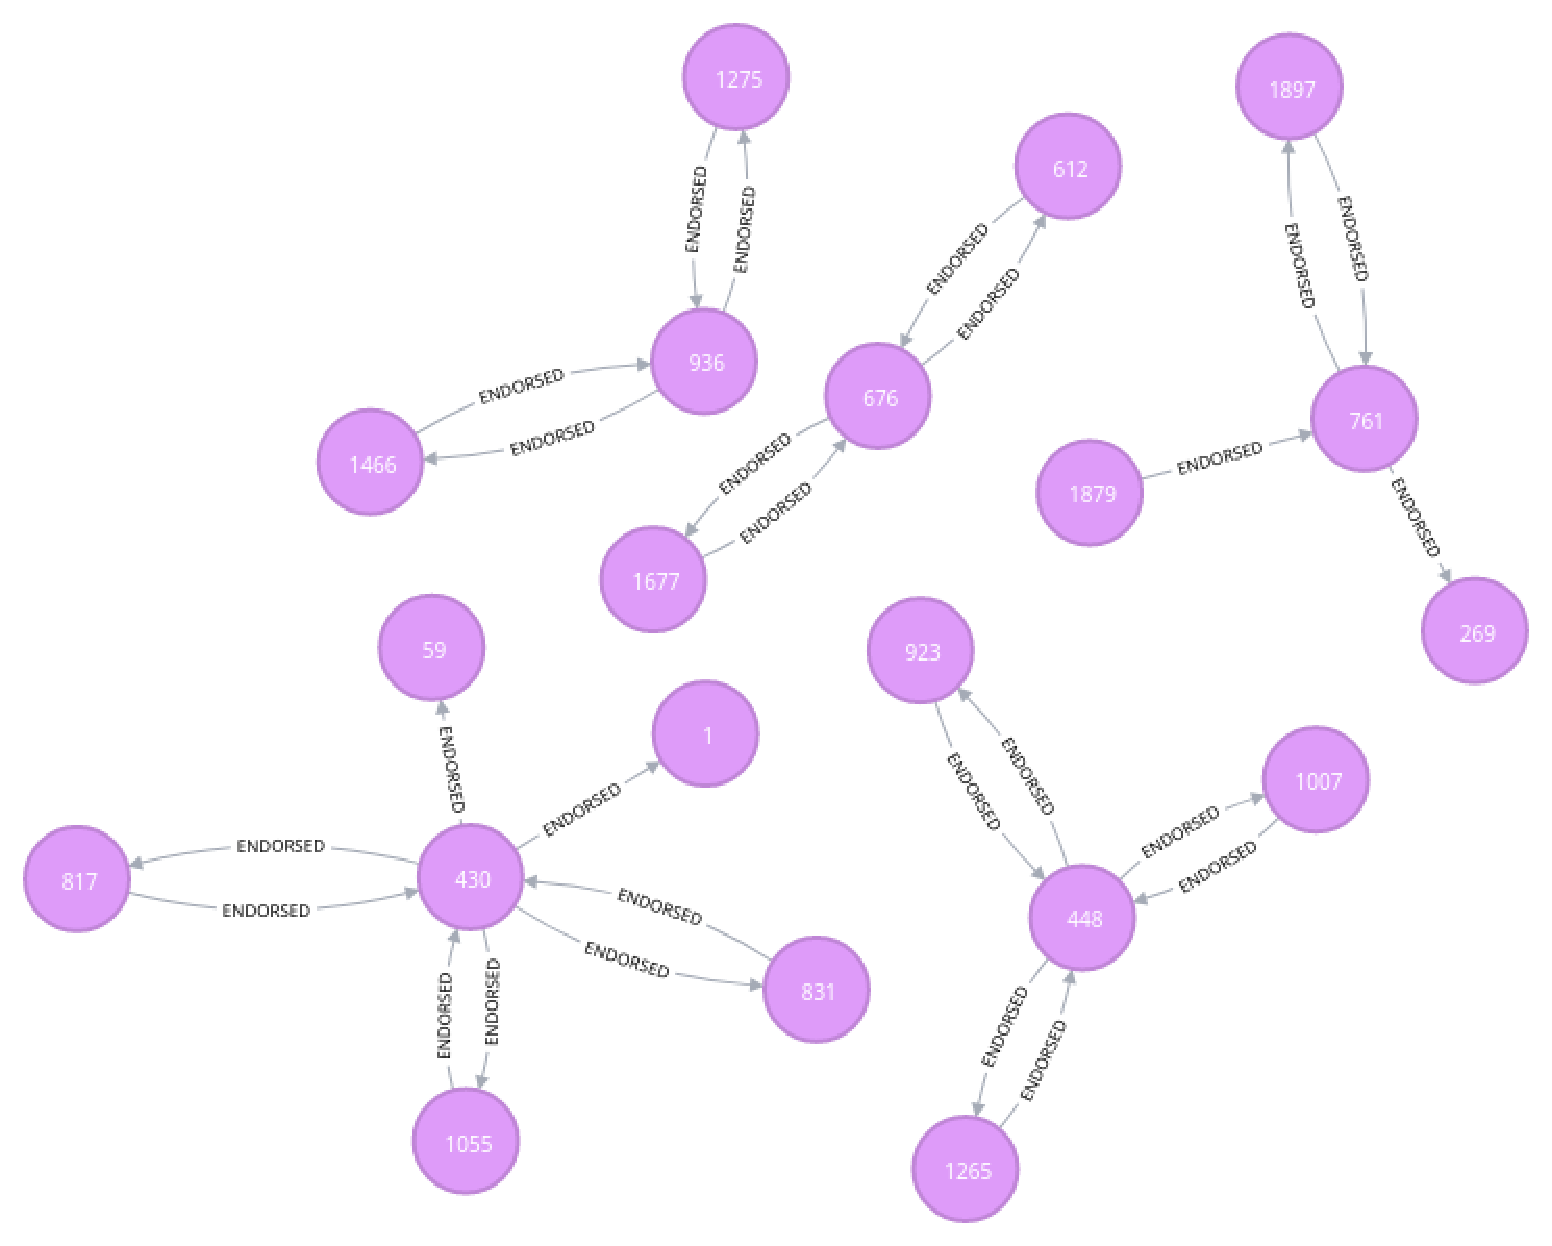
\includegraphics[width=0.95\textwidth]{Images/nodesWithImpactZero.eps}
	\caption{Interaction subgraph of nodes with zero impact}
	\label{fig:zeroimpact}
\end{figure}
\paragraph{Total Received Points:}Among the remaining 502 nodes, there were 5
nodes whose \ac{TEI} score was zero despite having more than one
incoming/outgoing connections. This value was because of \ac{TRP}, which is
another significant factor that the endorsement system takes into account.
Though the nodes received endorsements to have a considerable amount of
\ac{nER}, their \ac{TRP} was zero because their endorsers were not impactful
(i.e., having a \ac{TEI} score greater than zero or a \ac{nEG} or  \ac{nER}
score greater than one) in the network. The interaction subgraph for these five
no-
\begin{center} 
	\label{table:receivedpoints}
	\begin{tabularx}{\textwidth}{| X | X | X | X | X | X |} 
	\hline
  \textbf{Node label} & \textbf{nEG} & \textbf{nER} & \textbf{ratio} & \textbf{TRP} & \textbf{TEI} \\
  \hline 
  430  & 5 & 3 & 0.6 & 0 & 0  \\
  \hline
   761 & 2 & 2 & 1 & 0 & 0 \\
  \hline
  448 & 3 & 3 & 1 & 0 & 0 \\
  \hline
  676 & 2 & 2 & 1 & 0 & 0 \\
  \hline
  936 & 2 & 2 & 1 & 0 & 0 \\
  \hline
  \caption{Nodes with zero impact because of a non-impactful endorsers}
\end{tabularx}
\end{center}
\vspace{-15mm}
des is given by Figure~\ref{fig:zeroimpact}. As we can see from the figure,
none of the endorsers for these five nodes have a significant number of
connections for being an impactful node. This factor \ac{TRP} corresponds to
the prestige centrality metrics of a graph network where the significance of
adjacent nodes determines the significance of a node. In this case, the
significance of a node is not directly associated with \ac{TEI} of the endorser
but the value of \ac{CP} of each endorser that accumulatively contributes to
\ac{TRP} for the respective node. Table~\ref{table:receivedpoints} shows the
\ac{TRP} values across all the factors for these five nodes that explains why
the \ac{TRP} is zero which leads to them having a \ac{TEI} score of zero too. 
%\begin{figure}
%	\includegraphics[width=1.0\textwidth]{Images/TRPVsTEIFontSize.eps}
%	\caption{TRP vs. Total EDS Point}
%	\label{fig:receivedpointsvsimpact}
%\end{figure}

%\begin{figure}
%	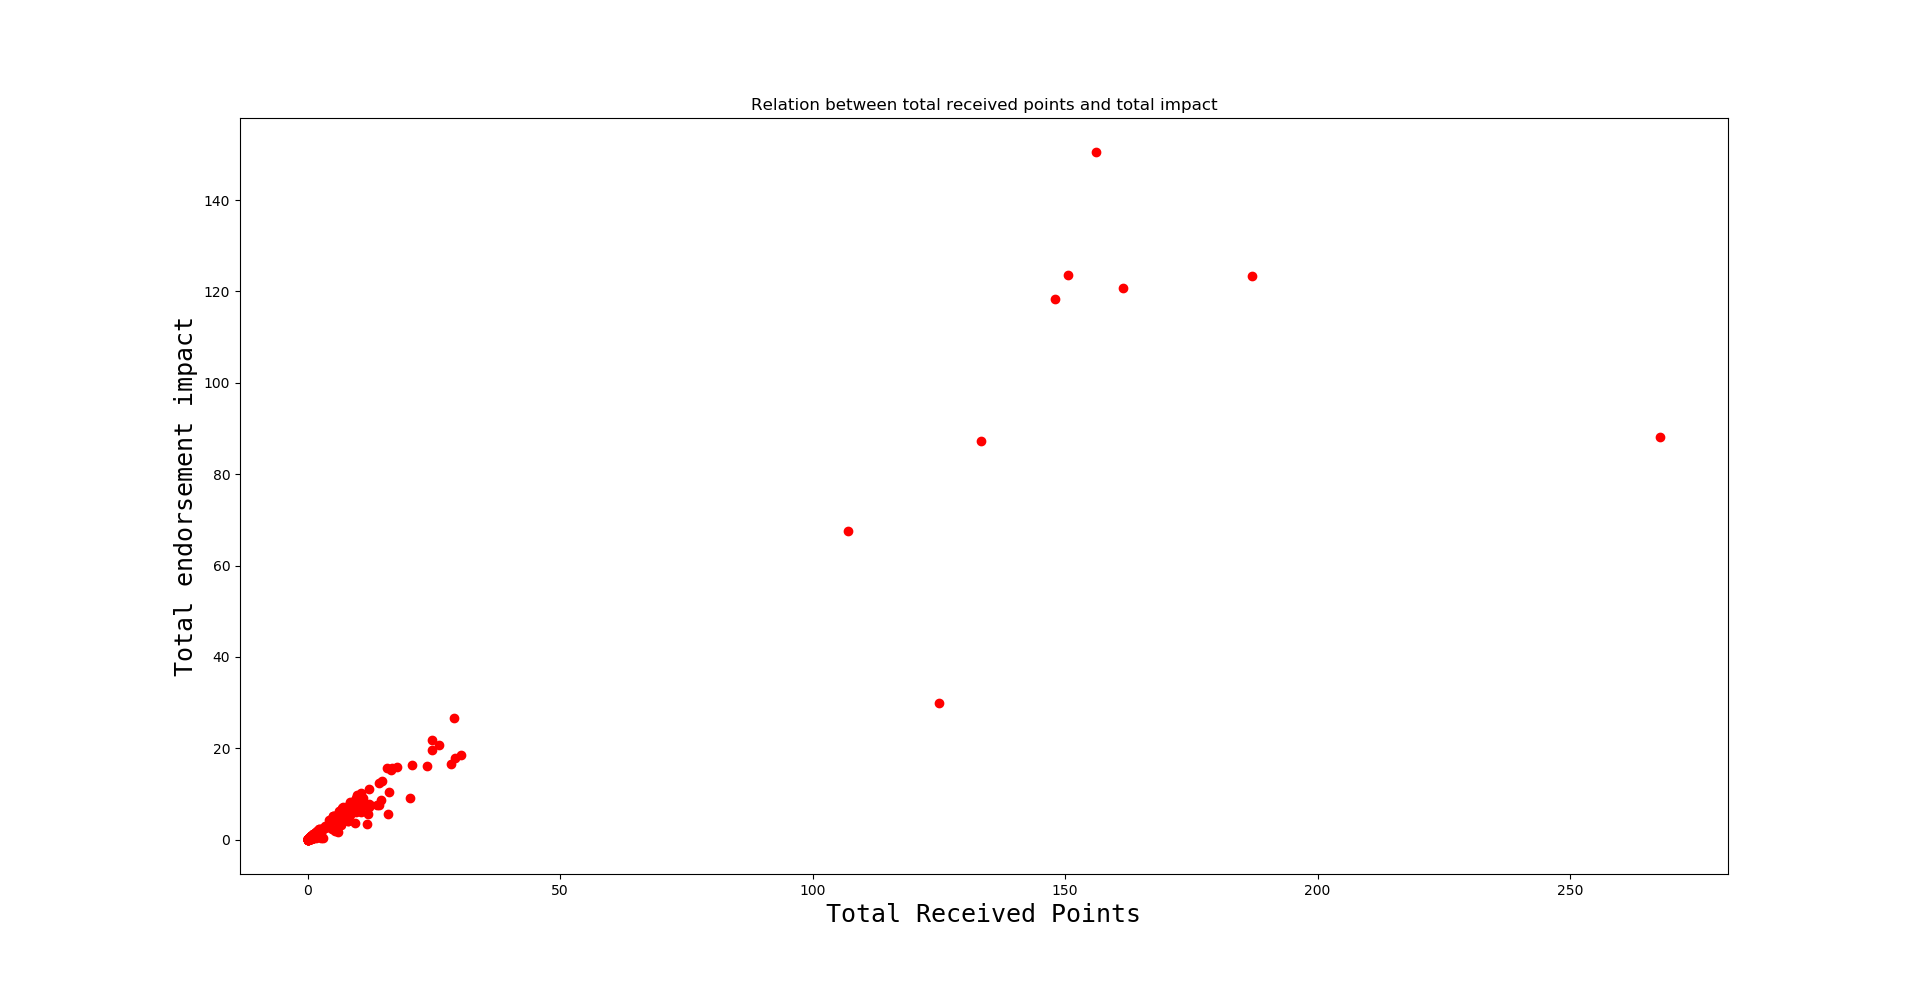
\includegraphics[width=1.0\textwidth]{Images/receivedPoints_impact_impactAboveZero.eps}
%	\caption{Received Points Vs. Total Endorsement Impact}
%	\label{fig:receivedpointvsimpact}
%\end{figure}
\paragraph{Ratio:} \label{par:ratio}
%\begin{figure}[H]
%	\includegraphics[width=0.95\textwidth]{Images/ratioVSimpact.eps}
%	\caption{Relation between Ratio and Total Endorsement Impact \ac{TEI}}
%	\label{fig:ratioimpact}
%\end{figure}
\begin{figure}[H]
	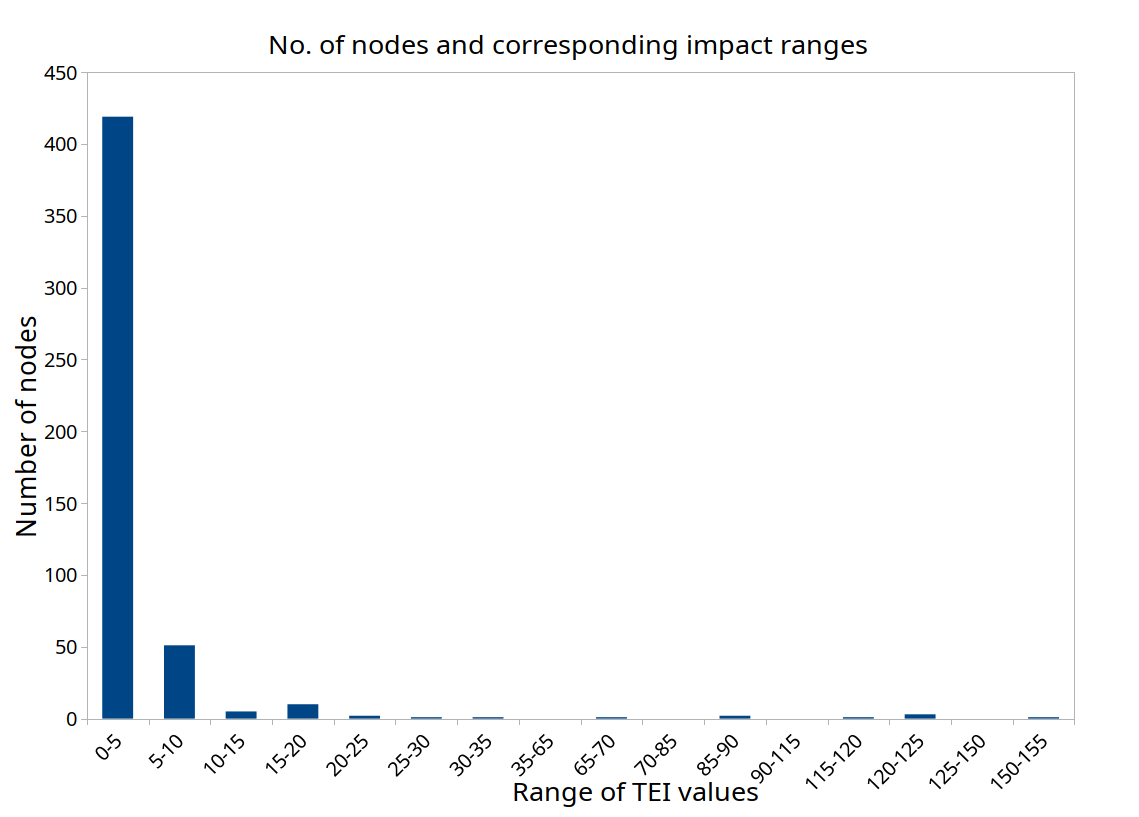
\includegraphics[width=1.0\textwidth]{Images/TEIRangesScaled.eps}
	\caption{Distribution of \ac{TEI} score over all nodes}
	\label{table:totalimpact}
\end{figure}
As we can see in Table~\ref{table:receivedpoints} that some nodes have a
maximum possible value of the ratio which is 1 and still has the lowest
~\ac{TEI} score. It shows that maintaining the ratio between incoming and
outgoing connections alone is not enough to have a significant impact on the
network. As such, it is difficult to say if a node is impactful or not merely
by looking at the ratio. A node that has a good ratio does not necessarily
imply that it has a good \ac{TEI} but a node with a good \ac{TEI} value should
have a higher ratio (value equal or approaching 1). This aspect is discussed in
more detail by Section~\ref{Allcases}. \par The distribution of \ac{TEI} score
over all nodes is given by Figure~\ref{table:totalimpact}. As the endorsement
system follows the ranking mechanism to rank the trustworthiness of nodes, the
higher the value of \ac{TEI} score higher is the trustworthiness of the given
node. We can see in Figure~\ref{table:totalimpact} that most of the nodes
have a lower impact value, i.e., about 400 of the nodes have the \ac{TEI} in
the range of 0-5. On the other hand, very few nodes have a high impact value,
i.e., about 1\% of the total nodes have \ac{TEI} score above the range of 100.
Thus, these few nodes can be considered relatively much trustworthy than any
other nodes in the network. The nodes labeled 4 and 2 in
Figure~\ref{fig:highImpactNode} shows the interaction behavior of nodes with
high \ac{TEI} score. 
%Section~\ref{subsec:bcConsensus}, they can be termed as a group of reputable
%nodes to sign and commit the block of transactions or to use as some set of
%pre-trusted nodes that can dynamically change based on more interactions. The
%ranking of nodes based on the impact value can be made. Higher the value of
%\ac{TEI} that a node has, higher is its trustworthiness. The
%Figure~\ref{fig:highImpactNode} shows the interaction graph structure of
%impactful node for the given nodes. As shown by the Figure, the high impact
%node has a significant amount of connections (incoming and outgoing) to have
%both the ratio and \ac{TRP} factor balanced.
%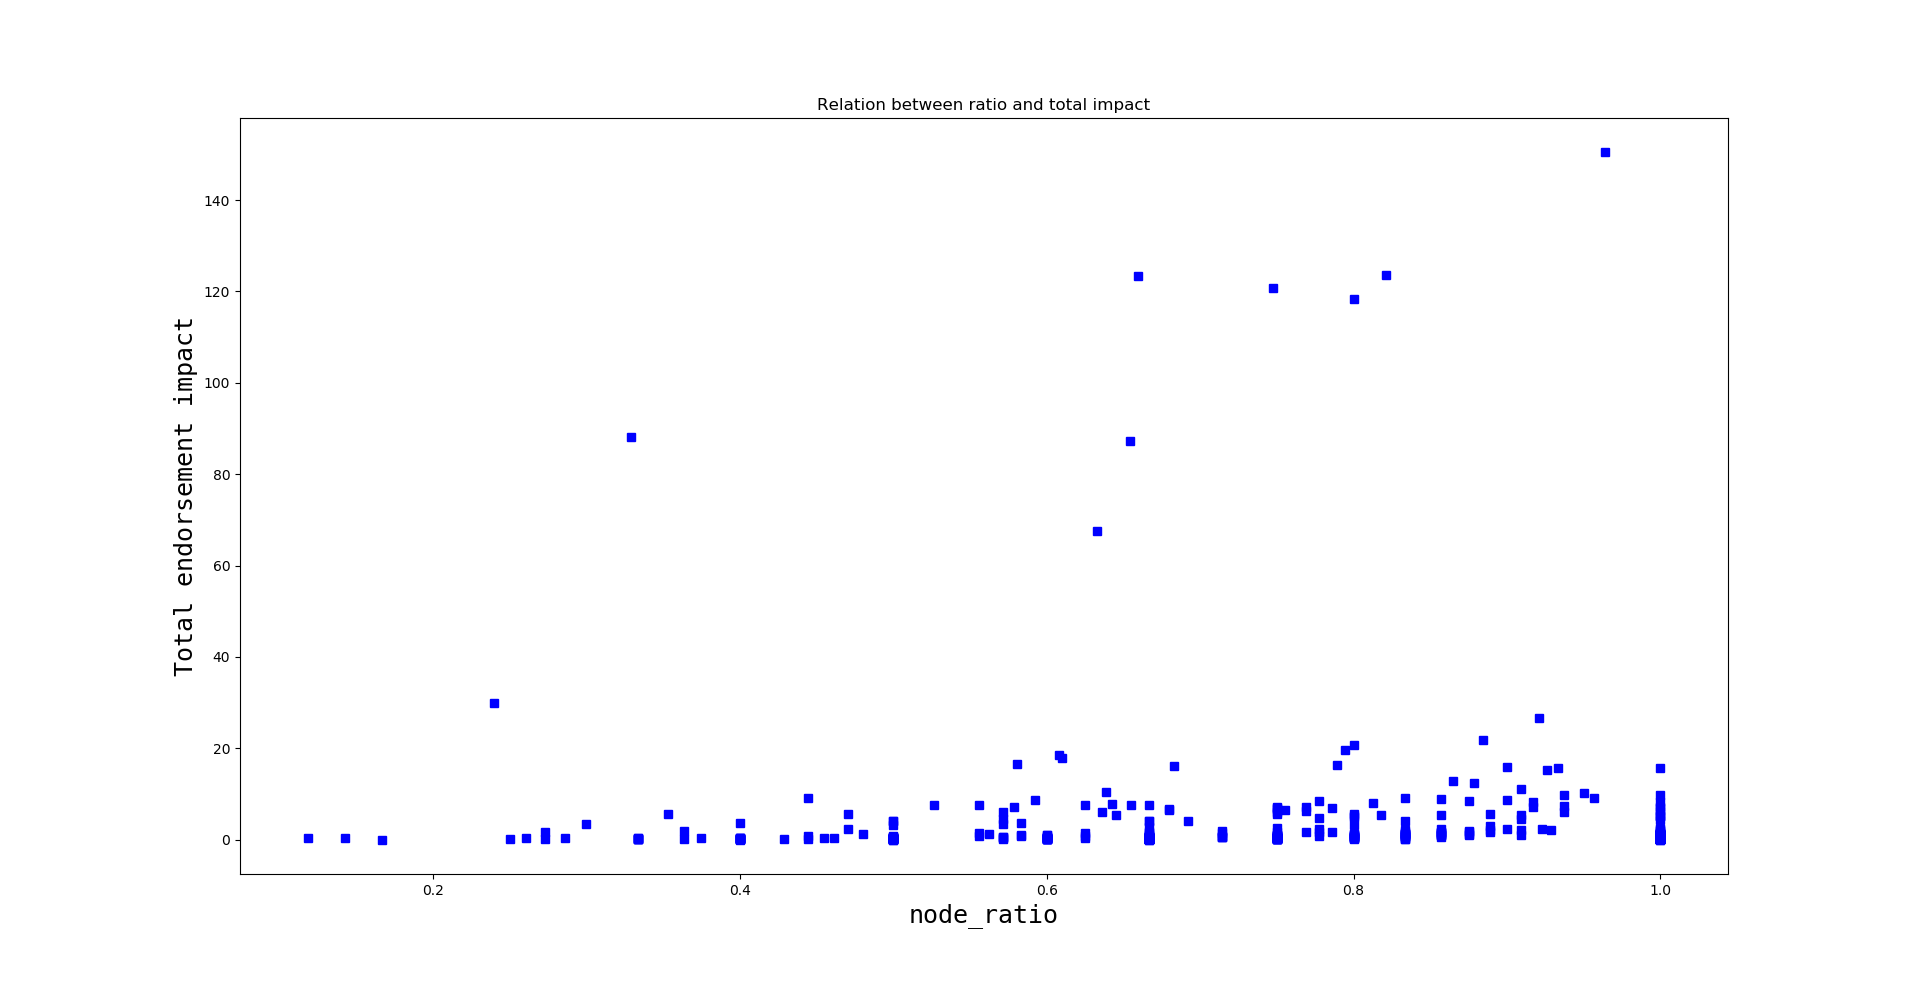
\includegraphics[width=0.95\textwidth]{Images/ratio_impact_impactAboveZero.eps}
\begin{figure}
	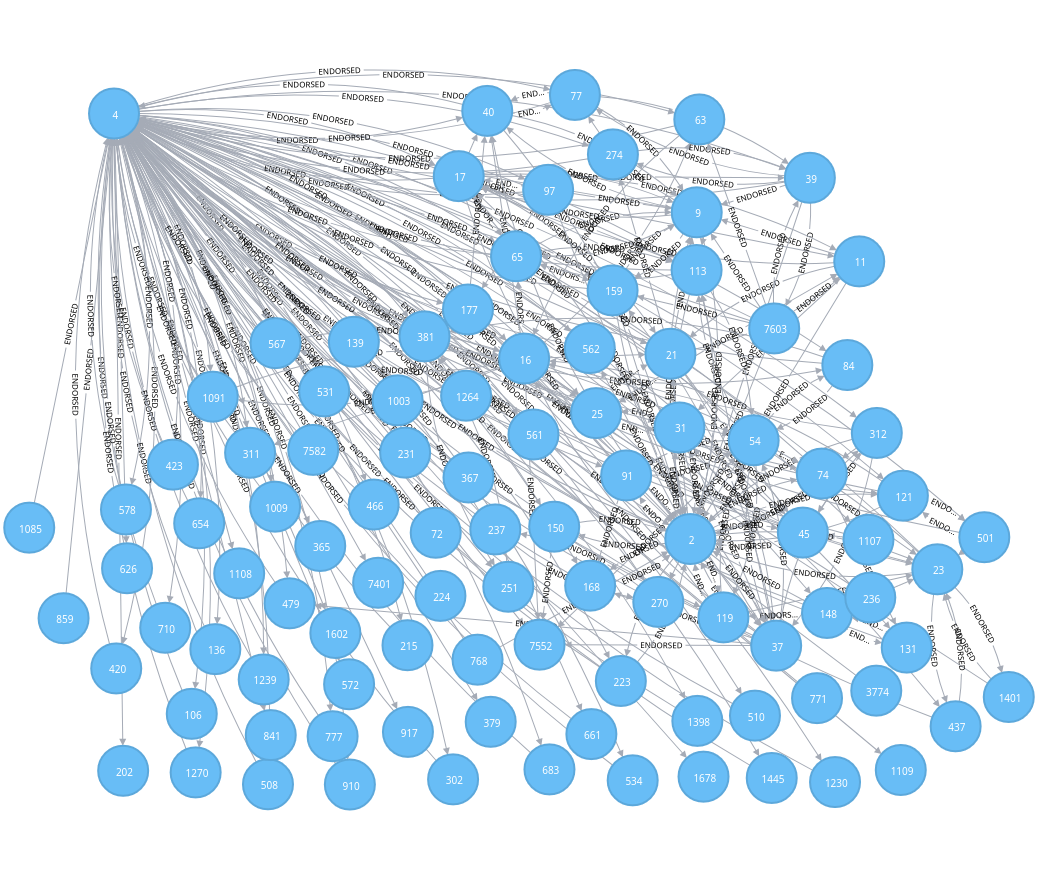
\includegraphics[width=1.0\textwidth]{Images/HighImpact_Node4.eps}
	\caption{Interaction of nodes (labeled 2 and 4) with higher \ac{TEI} score}
	\label{fig:highImpactNode}
\end{figure}
%\begin{tabularx}{\textwidth}{| X | X | }
%  \hline
%   \textbf{No. of nodes} & \textbf{Impact Range} \\
%  \hline 
%  419  & 0-5  \\
%  \hline
%   51 & 5-10 \\
%  \hline
%  5 & 10-15 \\
%  \hline
%  10 & 15-20 \\
%  \hline
%  2 & 20-25 \\
%  \hline
%  1 & 25-30 \\
%  \hline
%  1 & 30-35 \\
%  \hline
%  0 & 35-65 \\
%  \hline
%  1 & 65-70 \\
%  \hline
%  0 & 70-85 \\
%  \hline
%  2 & 85-90 \\
%  \hline
%  0 & 90-115 \\
%  \hline
%  1 & 115-120 \\
%  \hline
%  3 & 120-125 \\
%  \hline
%  0 & 125-150 \\
%  \hline
%  1 & 150-155 \\
%  \hline
%  \caption{No. of nodes and the corresponding impact ranges}
%  \label{table:totalimpact}
%\end{tabularx}
\section{Total impact across several factors with different
scenarios}\label{Allcases}
This section considers different scenarios to see how all the factors of the
endorsement system ( \ac{nEG}, \ac{nER}, ratio, \ac{TRP}, \ac{TEI} ) are
distributed for both high impact and low impact nodes. We have seen earlier
that a high or low value of the ratio is not a useful measure to distinguish
between a high impact or low impact node. Additionally, we also claimed that
even though a high ratio value does not imply a high impact node, a high impact
node should have a higher ratio (value equal to or approaching 1 and not
approaching 0). Thus, we will consider four different scenarios here to test
this behavior. The first two case takes a look at the node with a maximum
impact value whereas the last two case (case 3 and case 4) looks at the node
with a minimum impact value.
%This section considers different scenarios to analyze how several factors such
%as~\ac{nEG},~\ac{nER}, ratio,~\ac{TRP} is distributed and what contributes to
%having a higher or a lower~\ac{TEI} value. The first two case looks at the
%nodes that have maximum impact value on the network. As mentioned earlier, a
%node that does not have a maintained ratio (close to 1) cannot have a higher
%impact value. As such, it is interesting to see the minimum ratio that a high
%impact node can have. Case 1 and Case 2 does the same analysis to see the
%distribution of values across all the factors for a low impact node. The
\begin{figure}[h]
	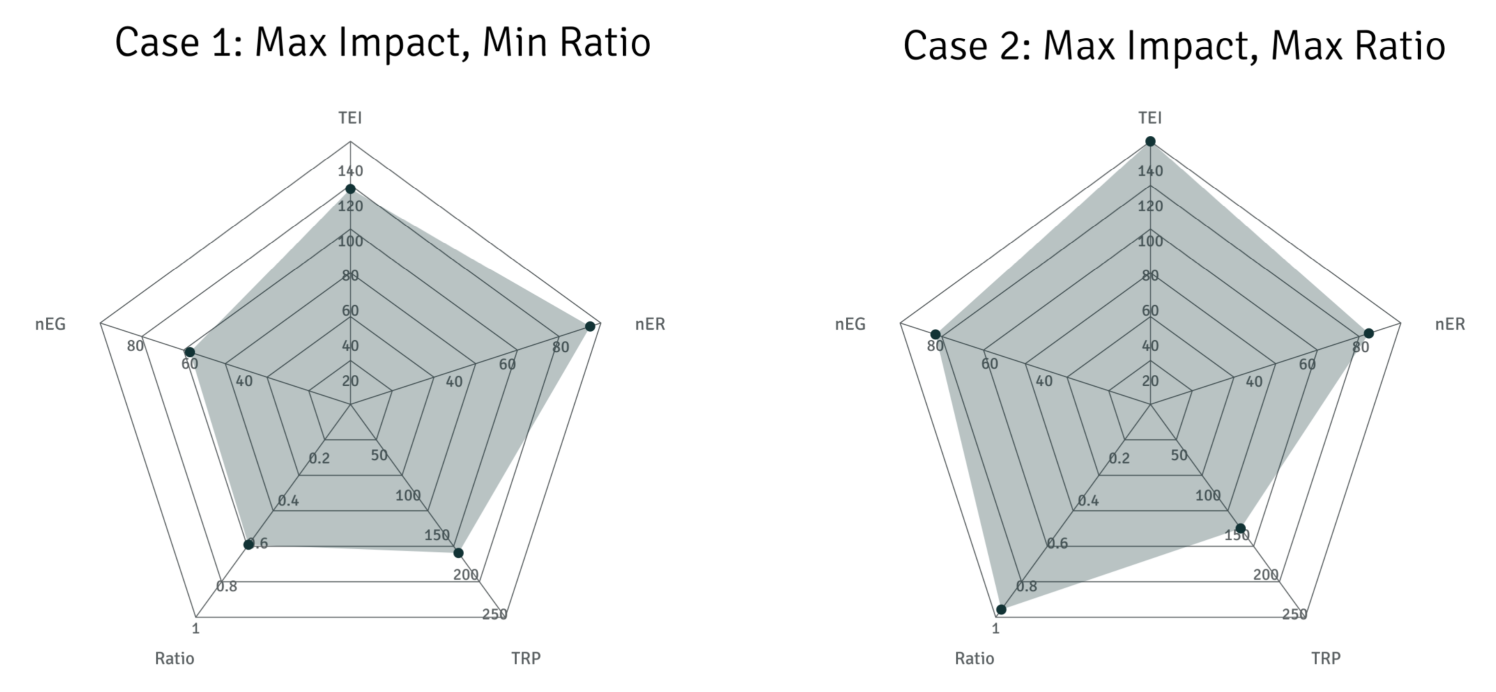
\includegraphics[width=1.1\textwidth]{Images/Case1andCase2.eps}
	\caption{High impact node with maximum and minimum possible ratio}
	\label{fig:case1andcase2}
\end{figure}
\paragraph{Case 1 \& Case 2: Maximum impact nodes}Here, we take the nodes that
have a higher range of impact values and among them take the node that has the
lowest ratio to depict case 1 and a node that has the highest ratio to depict
case 2. We can see both these cases and their distribution across other factors
in Figure~\ref{fig:case1andcase2}. The lowest ratio for case 1 is 0.6 (value
approaching 1) which is an expected value for a node with high impact.
Similarly, for case 2, we see that the maximum ratio is 1 which is also
expected as this node has the highest \ac{TEI} score. We can see in the figure
that for a high impact node, all other factors are almost evenly distributed
and based on their value of \ac{nEG} and \ac{nER} (above 60 in both cases ), we
can say that they have a high degree centr-
\begin{figure}[H]
	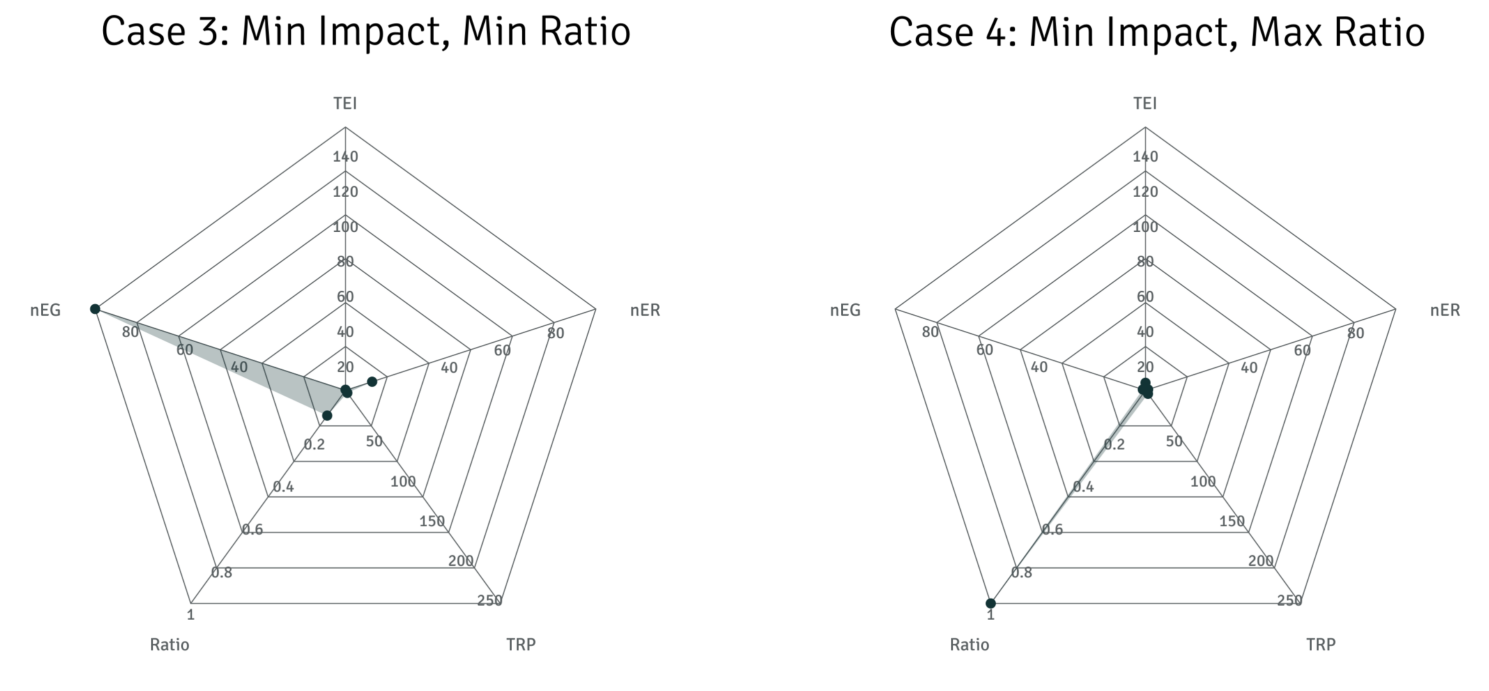
\includegraphics[width=1.1\textwidth]{Images/Case3andCase4.eps}
	\caption{Low impact node with maximum and minimum possible ratio}
	\label{fig:case3andcase4}
\end{figure}
ality as was shown by Figure~\ref{fig:highImpactNode} in
Section~\ref{par:ratio}. Therefore, they satisfy the requirement of being an
impactful node in the network.
\paragraph{Case 3 \& Case4: Minimum impact nodes}This scenario is the same as
the first two cases, except here we take the node with low impact values. We
can see the distribution across all factors for these nodes in
Figure~\ref{fig:case3andcase4}. Based on our earlier assumption about the
relation between ratio and \ac{TEI}, these nodes can have a maximum ratio
despite having a low \ac{TEI} score. We can see from the figure that case 3 has
too many outgoing connections but relatively very few incoming connections. As
such the minimum possible ratio for this node is also lower, i.e., it
approaches zero. Similarly, case 4 shows the maximum possible ratio of a low
impact node which is 1. Given that the node does not have enough incoming and
outgoing connections yet, it cannot have a very high impact value and therefore
its \ac{TEI} value is negligible. The third case shows the behavior of a node
that shows an extreme one-way connection whereas case 4 shows the behavior of
the starting node. As such, the low impact made by these nodes are expected. 
%\section{Summary of Results}

%\section{Blockchain: Gas Consumption, Block size, Transactions}
%Ethereum  specific concepts:
%As mentioned earlier, executing any operation on Ethereum costs some amount of
%gas. The total amount of transactions that can be included in an Ethereum block
%is therefore not determined by the size but by the amount of gas consumed by
%them. The block limitation is about 4 million gas per block.  The current block
%according to etherscan\footnote{http://etherscan.io/} is Block number 5778648
%with a total of 155 transactions recorded in it. The time between the previous
%block and the current block is around 11 seconds. Thus, the network throughput
%based on this data is around 11 transaction per second. The average block time is 17 seconds which is dynamically adjusted based on how fast or slow 
%





%The gas consumption for the transactions in endorsement contract is based on
%the tests performed on Rinkeby test network and remix environment. The gas
%price and gas limit are based on the statistics from the main ethereum network
%\footnote{https://ethgasstation.info/index.php}. The gas cost to join the
%endorsement network is 142927 units of gas and to send an endorsement is 203746
%units of gas. Recommended safe low value for the gas price is 2
%Gwei(0.000000002 eth). 
%The block size limitation in ethereum is about 4 million gas per block.
%Therefore, the total amount of transactions is not determined by its size but
%by the amount of gas it consumes. The current block according to
%etherscan\footnote{http://etherscan.io/} is Block number 5778648 with a total
%of 155 transactions recorded in it. The time between the previous block and the
%current block is around 11 seconds. Thus, the network throughput based on this
%data is around 11 transaction per second. 










%\section{Analysis}
%\section{Measurement}
%\section{Comparison}

% Presentation of results and case-study data 
% An application of the methodology is unfolded and results are presented using for example via Charts, Diagrams, Figures and Tables 
% The work is conducted in accordance with the method described earlier. Results are presented in an analytical way.
